\documentclass[a4paper]{article}

\usepackage[english]{babel}
\usepackage[utf8]{inputenc}
\usepackage{amsmath}
\usepackage{graphicx}
\usepackage[colorinlistoftodos]{todonotes}

\title{Advanced Networking Lab 4: MPLS}

\author{Péter Prjevara \& Kotaiba Alachkar}



\date{\today}

\begin{document}
\maketitle


\section{Task 1 - Discover the Topology}
\label{sec:task1}


\subsection{Task 1: Hand in the topology with the details filled in. It should be possible to rebuild the network from scratch using your diagram (while already knowing how to configure a juniper router of course).}

We must display the following: \textbf{addresses, prefixes, interface details, routing protocol, etc.}.


\begin{figure}[h]
\centering
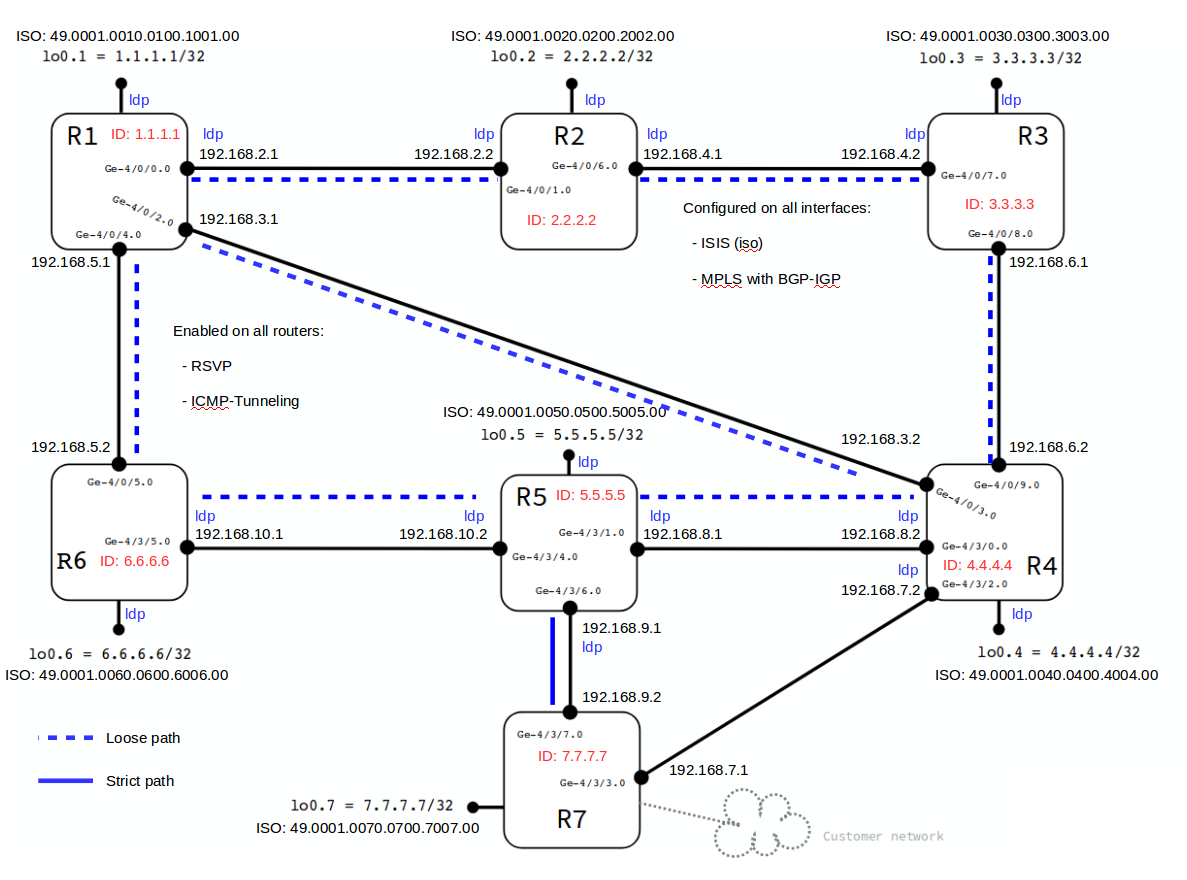
\includegraphics[width=1\textwidth]{topology.png}
\caption{\label{fig:topology_diagram}Detailed Topology Diagram}
\end{figure}


%ISIS ISO address format:

%https://ieoc.com/discussion/26360/isis-net-address-format

%https://www.cisco.com/c/en/us/td/docs/ios-xml/ios/iproute_isis/configuration/15-mt/irs-15-mt-book/irs-ovrw-cf.pdf

\section{Task 2 - Discover the Topology}
\label{sec:task2}


\subsection{Question 1 - How is MPLS configured on the routers? Which commands were used to set it up?}

In order to configure MPLS on the routers, first we enable MPLS on all the router interfaces:\\

\textbf{Then, MPLS enabled on all interfaces for each router.} Example configuration on router 1:


\begin{verbatim}

set logical-systems R1 interfaces ge-4/0/0 unit 0 family mpls
set logical-systems R1 interfaces ge-4/0/2 unit 0 family mpls
set logical-systems R1 interfaces ge-4/0/4 unit 0 family mpls
\end{verbatim}


\textbf{Then MPLS protocol is enabled on logical-systems on routers} (Some have with path configured and some without). ICMP tunneling is enabled on all interfaces, for debugging purposes. \footnote{http://66.129.228.18/documentation/en_US/junos12.1/topics/usage-guidelines/mpls-configuring-icmp-message-tunneling.html}

Path not configured example configuration:

\begin{verbatim}
set logical-systems R2 protocols mpls icmp-tunneling
set logical-systems R2 protocols mpls interface all

set logical-systems R5 protocols mpls icmp-tunneling
set logical-systems R5 protocols mpls interface all

set logical-systems R7 protocols mpls icmp-tunneling
set logical-systems R7 protocols mpls interface all  
    
\end{verbatim}


\begin{verbatim}
Path configured example configuration:


set logical-systems R1 protocols mpls traffic-engineering bgp-igp
set logical-systems R1 protocols mpls icmp-tunneling
set logical-systems R1 protocols mpls label-switched-path toR6 to 6.6.6.6
set logical-systems R1 protocols mpls label-switched-path toR6 ldp-tunneling
set logical-systems R1 protocols mpls label-switched-path toR6 no-cspf
set logical-systems R1 protocols mpls label-switched-path toR7 to 7.7.7.7
set logical-systems R1 protocols mpls label-switched-path toR7 install 145.125.0.0/24 active
set logical-systems R1 protocols mpls label-switched-path toR7 bandwidth 500m
set logical-systems R1 protocols mpls label-switched-path toR7 no-cspf
set logical-systems R1 protocols mpls label-switched-path toR7 primary VISIT-R5
set logical-systems R1 protocols mpls path VISIT-R5 5.5.5.5 loose
set logical-systems R1 protocols mpls interface all

set logical-systems R3 protocols mpls icmp-tunneling
set logical-systems R3 protocols mpls label-switched-path toR4 to 4.4.4.4
set logical-systems R3 protocols mpls label-switched-path toR4 ldp-tunneling
set logical-systems R3 protocols mpls label-switched-path toR4 no-cspf
set logical-systems R3 protocols mpls interface all

set logical-systems R4 protocols mpls icmp-tunneling
set logical-systems R4 protocols mpls label-switched-path toR3 to 3.3.3.3
set logical-systems R4 protocols mpls label-switched-path toR3 ldp-tunneling
set logical-systems R4 protocols mpls label-switched-path toR3 no-cspf
set logical-systems R4 protocols mpls interface all

set logical-systems R6 protocols mpls icmp-tunneling
set logical-systems R6 protocols mpls label-switched-path toR1 to 1.1.1.1
set logical-systems R6 protocols mpls label-switched-path toR1 ldp-tunneling
set logical-systems R6 protocols mpls label-switched-path toR1 no-cspf
set logical-systems R6 protocols mpls interface all

\end{verbatim}



\subsection{Question 2 - Which routing protocol is configured? List the relevant details from the configuration for that protocol and explain what they mean?}

The routing protocol that configured is \textbf{IS-IS}. The relevant details from the configuration for Router 1:

\begin{verbatim}
set logical-systems R1 interfaces ge-4/0/0 unit 0 family iso
set logical-systems R1 interfaces ge-4/0/2 unit 0 family iso
set logical-systems R1 interfaces ge-4/0/4 unit 0 family iso
set logical-systems R1 interfaces lo0 unit 1 family iso address 49.0001.0010.0100.1001.00
set logical-systems R1 protocols isis overload timeout 100
set logical-systems R1 protocols isis level 1 disable
set logical-systems R1 protocols isis level 2 wide-metrics-only
set logical-systems R1 protocols isis interface ge-4/0/0.0 point-to-point
set logical-systems R1 protocols isis interface ge-4/0/2.0 point-to-point
set logical-systems R1 protocols isis interface ge-4/0/4.0 point-to-point
set logical-systems R1 protocols isis interface lo0.1 passive
\end{verbatim}


\subsubsection{Explanation of commands}

Following command on all routers means (own IS-IS address) It contains the following Area Address, System ID, and NSAP Selector.

\begin{verbatim}
    Example: set logical-systems R1 interfaces lo0 unit 1 family iso address 49.0001.0010.0100.1001.00
\end{verbatim}

Following command on all routers means that the specific interface is able to receive ISIS PDUs.

\begin{verbatim}
    set logical-systems R# interfaces ge-4/X/X unit Z family iso 
\end{verbatim}


Following command on all routers means the router would advertise max metric for a duration of 100 sec after the router startup.

\begin{verbatim}    
    set logical-systems R# protocols isis overload timeout 100
\end{verbatim}

ISIS can be working on multiple (two) levels. This is to support protocol stability: the different levels are segregated, such like OSPF areas. In this particular case, all routers are configured to be level 2 routers, as the topology isn't so complicated.

%Following command on all routers means Disable IS-IS on the routing device, on an interface, or on a level. By default, IS-IS is enabled for IS-IS areas on all interfaces on which the ISO protocol family is enabled. To disable IS-IS at any particular level on an interface, include the disable statement.

\begin{verbatim}
     set logical-systems R# protocols isis level 1 disable
\end{verbatim}



Following command on all routers means to configure IS-IS to generate only the new pair of TLVs instead of the originals, and thus allow a wider range of metric values suitable for traffic engineering. When wide-metrics-only is configured for a level, Junos suppresses the generation of narrow-style-metric TLV`s, imporving performance.

\begin{verbatim}    
    set logical-systems R# protocols isis level 2 wide-metrics-only
\end{verbatim}

Following command on all routers means configure an IS-IS interface to behave like a point-to-point connection. You can use the point-to-point statement to configure a LAN interface to act like a point-to-point interface for IS-IS.

\begin{verbatim}    
    set logical-systems R# protocols isis interface ge-4/X/X.0 point-to-point
\end{verbatim}


The following command effectively prevents IS-IS from running on the interface. \textit{This command is configured on all the loopback interfaces, where it is unnecessary to run routing.}

\begin{verbatim}    
    set logical-systems R# protocols isis interface lo0.X passive
\end{verbatim}


Following command means that the Logical system R7 has an additional policy statement. It's used for exporting the static routes information into IS-IS:

\begin{verbatim}
    set logical-systems R7 protocols isis export putintoisis
    set logical-systems R7 policy-options policy-statement putintoisis term 1 from protocol static 
    set logical-systems R7 policy-options policy-statement putintoisis term 1 then accept
\end{verbatim}


\subsection{Question 3 - Between which routers are LDP sessions established? How is this configured? Which LSPs have been set up with LDP? List the relevant details of these LSPs to explain how you discovered this. (Pick one of the LSPs to explain all details about it.) Look at the label database and the FECs and check the routing table(s).}


The following LDP tunnels are configured within the system (these links are also not using LDP):

\begin{verbatim}
Router 1 >> Router 7 and Router 6
Router 3 >> Router 4
\end{verbatim}

This relationship is also depicted on the drawing at the beginning of this document. LDP distribution is configured between all the other interfaces of all the other routers, depicted by the following snippet from the configuration.


\begin{verbatim}
set logical-systems R1 protocols ldp interface ge-4/0/0.0
set logical-systems R1 protocols ldp interface lo0.1
set logical-systems R2 protocols ldp interface all
set logical-systems R3 protocols ldp interface ge-4/0/7.0
set logical-systems R3 protocols ldp interface lo0.3
set logical-systems R4 protocols ldp interface ge-4/3/0.0
set logical-systems R4 protocols ldp interface ge-4/3/2.0
set logical-systems R4 protocols ldp interface lo0.4
set logical-systems R5 protocols ldp interface all
set logical-systems R6 protocols ldp interface ge-4/3/5.0
set logical-systems R6 protocols ldp interface lo0.6
set logical-systems R7 protocols ldp interface all    
\end{verbatim}


\textbf{List the relevant details of these LSPs:}

\begin{verbatim}
    
student@chico:R1> show ldp session             
  Address           State        Connection     Hold time
2.2.2.2             Operational  Open             26
6.6.6.6             Operational  Open             21


student@chico:R2> show ldp session             
  Address           State        Connection     Hold time
1.1.1.1             Operational  Open             23
3.3.3.3             Operational  Open             29

student@chico:R3> show ldp session             
  Address           State        Connection     Hold time
2.2.2.2             Operational  Open             20
4.4.4.4             Operational  Open             25
    
student@chico:R4> show ldp session             
  Address           State        Connection     Hold time
3.3.3.3             Operational  Open             24
5.5.5.5             Operational  Open             24
7.7.7.7             Operational  Open             24

student@chico:R5> show ldp session             
  Address           State        Connection     Hold time
4.4.4.4             Operational  Open             29
6.6.6.6             Operational  Open             29
7.7.7.7             Operational  Open             29

student@chico:R6> show ldp session             
  Address           State        Connection     Hold time
1.1.1.1             Operational  Open             23
5.5.5.5             Operational  Open             28

student@chico:R7> show ldp session 
  Address           State        Connection     Hold time
4.4.4.4             Operational  Open             28
5.5.5.5             Operational  Open             28


\end{verbatim}


\textbf{The command used to configure LDP on interface is:}

\begin{verbatim}
    set logical-systems R# protocols ldp interface <interface number>
\end{verbatim}


The LDP sessions per logical system are the following:

\begin{verbatim}
Router 1 <<>> Router 2 and Router 6
Router 2 <<>> Router 3
Router 3 <<>> Router 4
Router 4 <<>> Router 5 and Router 7
Router 5 <<>> Router 6 and Router 7
\end{verbatim}



The LSPs toR2, toR3, toR4 and toR6 are configured with LDP:

\begin{verbatim}
set logical-systems R6 protocols mpls label-switched-path toR1 ldp-tunneling
set logical-systems R4 protocols mpls label-switched-path toR3 ldp-tunneling
set logical-systems R3 protocols mpls label-switched-path toR4 ldp-tunneling
set logical-systems R1 protocols mpls label-switched-path toR6 ldp-tunneling

LSP on Router 4:
set logical-systems R4 protocols mpls label-switched-path toR3 to 3.3.3.3
set logical-systems R4 protocols mpls label-switched-path toR3 ldp-tunneling
set logical-systems R4 protocols mpls label-switched-path toR3 no-cspf
\end{verbatim}

As we see above, The no-cspf command shows that the constrained-path LSP computation has been disabled. 



\textbf{The label database are the following}:

\begin{verbatim}
    student@chico:R4> show ldp database brief 
Input label database, 4.4.4.4:0--3.3.3.3:0
  Label     Prefix
 299808     1.1.1.1/32
 299776     2.2.2.2/32
      3     3.3.3.3/32
 299792     4.4.4.4/32
 299840     5.5.5.5/32
 299824     6.6.6.6/32
 299856     7.7.7.7/32

Output label database, 4.4.4.4:0--3.3.3.3:0
  Label     Prefix
 299824     2.2.2.2/32
 299776     3.3.3.3/32
      3     4.4.4.4/32
 299792     5.5.5.5/32
 299856     6.6.6.6/32
 299808     7.7.7.7/32

Input label database, 4.4.4.4:0--5.5.5.5:0
  Label     Prefix
 299872     1.1.1.1/32
 299840     2.2.2.2/32
 299824     3.3.3.3/32                  
 299792     4.4.4.4/32
      3     5.5.5.5/32
 299808     6.6.6.6/32
 299776     7.7.7.7/32

Output label database, 4.4.4.4:0--5.5.5.5:0
  Label     Prefix
 299824     2.2.2.2/32
 299776     3.3.3.3/32
      3     4.4.4.4/32
 299792     5.5.5.5/32
 299856     6.6.6.6/32
 299808     7.7.7.7/32

Input label database, 4.4.4.4:0--7.7.7.7:0
  Label     Prefix
 299824     2.2.2.2/32
 299808     3.3.3.3/32
 299792     4.4.4.4/32
 299776     5.5.5.5/32
 299840     6.6.6.6/32
      3     7.7.7.7/32
                                        
Output label database, 4.4.4.4:0--7.7.7.7:0
  Label     Prefix
 299824     2.2.2.2/32
 299776     3.3.3.3/32
      3     4.4.4.4/32
 299792     5.5.5.5/32
 299856     6.6.6.6/32
 299808     7.7.7.7/32
\end{verbatim}

The previous output shows all labels and its corresponding to a specific destination.


\textbf{Now, routing table for Router 4:} This routing table shows the labels, including IP-addresses, destination and the LSP that is related to the specific route.


\begin{verbatim}
student@chico:R4> show route 

mpls.0: 12 destinations, 12 routes (12 active, 0 holddown, 0 hidden)
+ = Active Route, - = Last Active, * = Both

0                  *[MPLS/0] 1d 01:19:36, metric 1
                      Receive
1                  *[MPLS/0] 1d 01:19:36, metric 1
                      Receive
2                  *[MPLS/0] 1d 01:19:36, metric 1
                      Receive
299776             *[LDP/9] 1d 01:18:42, metric 1
                    > to 192.168.6.1 via ge-4/0/9.0, label-switched-path toR3
299776(S=0)        *[LDP/9] 1d 01:18:42, metric 1
                    > to 192.168.6.1 via ge-4/0/9.0, label-switched-path toR3
299792             *[LDP/9] 1d 01:18:17, metric 1
                    > to 192.168.8.1 via ge-4/3/0.0, Pop      
299792(S=0)        *[LDP/9] 1d 01:18:17, metric 1
                    > to 192.168.8.1 via ge-4/3/0.0, Pop      
299808             *[LDP/9] 1d 01:18:14, metric 1
                    > to 192.168.7.1 via ge-4/3/2.0, Pop      
299808(S=0)        *[LDP/9] 1d 01:18:14, metric 1
                    > to 192.168.7.1 via ge-4/3/2.0, Pop      
299824             *[LDP/9] 1d 01:17:55, metric 1
                    > to 192.168.6.1 via ge-4/0/9.0, label-switched-path toR3
299856             *[LDP/9] 1d 01:17:14, metric 1
                    > to 192.168.8.1 via ge-4/3/0.0, Swap 299808
299888             *[RSVP/7/1] 23:32:10, metric 1
                    > to 192.168.8.1 via ge-4/3/0.0, label-switched-path toR7

\end{verbatim}

The router-IDs or Loopback interface addresses are used as FEC. They are a set of prefixes treated similarly. 


\subsection{Question 4 - Which LSPs are configured with RSVP? How are they configured? Determine as many details about the LSPs as you are able to find?}

RSVP is enabled for all LSPs. RSVP  is enabled per interface but it is not specifically defined within the LSP.

LSPs are configures:

\begin{verbatim}
student@chico:R1> show rsvp session 
Ingress RSVP: 2 sessions
To              From            State   Rt Style Labelin Labelout LSPname 
6.6.6.6         1.1.1.1         Up       0  1 FF       -        3 toR6
7.7.7.7         1.1.1.1         Up       0  1 FF       -   299888 toR7
Total 2 displayed, Up 2, Down 0

Egress RSVP: 1 sessions
To              From            State   Rt Style Labelin Labelout LSPname 
1.1.1.1         6.6.6.6         Up       0  1 FF       3        - toR1
Total 1 displayed, Up 1, Down 0

Transit RSVP: 0 sessions
Total 0 displayed, Up 0, Down 0

student@chico:R2> show rsvp session 
Ingress RSVP: 0 sessions
Total 0 displayed, Up 0, Down 0

Egress RSVP: 0 sessions
Total 0 displayed, Up 0, Down 0

Transit RSVP: 0 sessions
Total 0 displayed, Up 0, Down 0


student@chico:R3> show rsvp session                          
Ingress RSVP: 1 sessions
To              From            State   Rt Style Labelin Labelout LSPname 
4.4.4.4         3.3.3.3         Up       0  1 FF       -        3 toR4
Total 1 displayed, Up 1, Down 0

Egress RSVP: 1 sessions
To              From            State   Rt Style Labelin Labelout LSPname 
3.3.3.3         4.4.4.4         Up       0  1 FF       3        - toR3
Total 1 displayed, Up 1, Down 0

Transit RSVP: 0 sessions
Total 0 displayed, Up 0, Down 0

student@chico:R4> show rsvp session            
Ingress RSVP: 1 sessions
To              From            State   Rt Style Labelin Labelout LSPname 
3.3.3.3         4.4.4.4         Up       0  1 FF       -        3 toR3
Total 1 displayed, Up 1, Down 0

Egress RSVP: 1 sessions
To              From            State   Rt Style Labelin Labelout LSPname 
4.4.4.4         3.3.3.3         Up       0  1 FF       3        - toR4
Total 1 displayed, Up 1, Down 0

Transit RSVP: 1 sessions
To              From            State   Rt Style Labelin Labelout LSPname 
7.7.7.7         1.1.1.1         Up       0  1 FF  299888   299904 toR7
Total 1 displayed, Up 1, Down 0


student@chico:R5> show rsvp session            
Ingress RSVP: 0 sessions
Total 0 displayed, Up 0, Down 0

Egress RSVP: 0 sessions
Total 0 displayed, Up 0, Down 0

Transit RSVP: 1 sessions
To              From            State   Rt Style Labelin Labelout LSPname 
7.7.7.7         1.1.1.1         Up       0  1 FF  299904        3 toR7
Total 1 displayed, Up 1, Down 0

student@chico:R6> show rsvp session            
Ingress RSVP: 1 sessions
To              From            State   Rt Style Labelin Labelout LSPname 
1.1.1.1         6.6.6.6         Up       0  1 FF       -        3 toR1
Total 1 displayed, Up 1, Down 0

Egress RSVP: 1 sessions
To              From            State   Rt Style Labelin Labelout LSPname 
6.6.6.6         1.1.1.1         Up       0  1 FF       3        - toR6
Total 1 displayed, Up 1, Down 0

Transit RSVP: 0 sessions
Total 0 displayed, Up 0, Down 0

student@chico:R7> show rsvp session            
Ingress RSVP: 0 sessions
Total 0 displayed, Up 0, Down 0

Egress RSVP: 1 sessions
To              From            State   Rt Style Labelin Labelout LSPname 
7.7.7.7         1.1.1.1         Up       0  1 FF       3        - toR7
Total 1 displayed, Up 1, Down 0

Transit RSVP: 0 sessions
Total 0 displayed, Up 0, Down 0

\end{verbatim}

RSVP Configurations:

\begin{verbatim}
set logical-systems R1 protocols rsvp interface all
set logical-systems R2 protocols rsvp interface all
set logical-systems R3 protocols rsvp interface all
set logical-systems R4 protocols rsvp interface all
set logical-systems R5 protocols rsvp interface all
set logical-systems R6 protocols rsvp interface all
set logical-systems R7 protocols rsvp interface all
\end{verbatim}



\section{Task 3 - Prepare the config to add a new router}
\label{sec:task3}


\subsection{Task 3: Give your prepared configuration for router R8. Including explanations for each command you use.}

\begin{verbatim}

x name of the router: R8
- R8 needs to be connected to R1 and R3 (see drawing next page)
x GE interfaces to be used on R8: Ge-4/3/8 and Ge-4/3/9
x Loopback address: 8.8.8.8
- Assign prefixes to the links (pick appropriately sized subnets)
x R8 should become part of the MPLS core
x R8 must run LDP
- An RSVP signalled LSP to R6 with reserved bandwidth of 200M should be built
- Another RSVP LSP to R4 with reserved bandwidth of 300M should be built


The configuration for R8 only:

set logical-systems R8 interfaces ge-4/3/8 unit 0 family inet address 192.168.2.2/30
set logical-systems R8 interfaces ge-4/3/8 unit 0 family iso
set logical-systems R8 interfaces ge-4/3/8 unit 0 family mpls

set logical-systems R8 interfaces ge-4/3/9 unit 0 family inet address 192.168.4.1/30
set logical-systems R8 interfaces ge-4/3/9 unit 0 family iso
set logical-systems R8 interfaces ge-4/3/9 unit 0 family mpls

set logical-systems R8 interfaces lo0 unit 2 family inet address 8.8.8.8/32 primary
set logical-systems R8 interfaces lo0 unit 2 family iso address 49.0001.0080.0800.8008.00

set logical-systems R8 protocols rsvp interface all

set logical-systems R8 protocols mpls icmp-tunneling
set logical-systems R8 protocols mpls interface all

set logical-systems R8 protocols isis overload timeout 100
set logical-systems R8 protocols isis level 1 disable
set logical-systems R8 protocols isis level 2 wide-metrics-only
set logical-systems R8 protocols isis interface ge-4/3/8.0 point-to-point
set logical-systems R8 protocols isis interface ge-4/3/9.0 point-to-point
set logical-systems R8 protocols isis interface lo0.8 passive
set logical-systems R8 protocols ldp interface all
set logical-systems R8 routing-options router-id 8.8.8.8
set logical-systems R8 protocols mpls label-switched-path toR4 to 3.3.3.3 bandwidth 300m
set logical-systems R8 protocols mpls label-switched-path toR4 ldp-tunneling
set logical-systems R8 protocols mpls label-switched-path toR6 to 3.3.3.3 bandwidth 200m
set logical-systems R8 protocols mpls label-switched-path toR6 ldp-tunneling
\end{verbatim}

\textbf{You can find the explanation for each command used at Task 2 section 2.2}


\end{document}